\documentclass[12pt,a4paper,openright,twoside]{book}
\usepackage[utf8]{inputenc}
\usepackage{disi-thesis}
\usepackage{code-lstlistings}
\usepackage{notes}
\usepackage{shortcuts}
\usepackage{acronym}
\school{\unibo}
\programme{Corso di Laurea Magistrale in Ingegneria e Scienze Informatiche}
\title{Fancy Title}
\author{Giacomo Accursi}
\date{\today}
\subject{Laboratorio di Sistemi Software}
\supervisor{Prof. Danilo Pianini}
\cosupervisor{Dott. Gianluca Aguzzi}
\session{IV}
\academicyear{2022-2023}

% Definition of acronyms
% \acrodef{IoT}{Internet of Thing}
% \acrodef{vm}[VM]{Virtual Machine}


\mainlinespacing{1.241}

\begin{document}

\frontmatter\frontispiece

\begin{abstract}	
Max 2000 characters, strict.
\end{abstract}

\begin{dedication} % this is optional
Optional. Max a few lines.
\end{dedication}

\begin{acknowledgements} % this is optional
Optional. Max 1 page.
\end{acknowledgements}

%----------------------------------------------------------------------------------------
\tableofcontents   
\listoffigures     % (optional) comment if empty
\lstlistoflistings % (optional) comment if empty
%----------------------------------------------------------------------------------------

\mainmatter

%----------------------------------------------------------------------------------------
\chapter{Introduction}
\label{chap:introduction}
%----------------------------------------------------------------------------------------

% Write your intro here.
% \sidenote{Add sidenotes in this way. They are named after the author of the thesis}

% You can use acronyms that your defined previously,
% such as \ac{IoT}.
% %
% If you use acronyms twice,
% they will be written in full only once
% (indeed, you can mention the \ac{IoT} now without it being fully explained).
% %
% In some cases, you may need a plural form of the acronym.
% %
% For instance,
% that you are discussing \acp{vm},
% you may need both \ac{vm} and \acp{vm}.

% \paragraph{Structure of the Thesis}

% \note{At the end, describe the structure of the paper}

% \chapter{State of the art}

% I suggest referencing stuff as follows: \cref{fig:random-image} or \Cref{fig:random-image}

% \begin{figure}
%     \centering
%     \includegraphics[width=.8\linewidth]{}
%     \caption{Some random image}
%     \label{fig:random-image}
% \end{figure}

% \section{Some cool topic}

% \chapter{Contribution}

% You may also put some code snippet (which is NOT float by default), eg: \cref{lst:random-code}.

% \lstinputlisting[float,language=Java,label={lst:random-code}]{listings/HelloWorld.java}


%----------------------------------------------------------------------------------------
% Discrete Event Simulation
%----------------------------------------------------------------------------------------
\chapter{Simulazioni ad Eventi Discreti}
\section{Panoramica sulle simulazioni ad eventi discreti}
Un sistema ad eventi discreti è un sistema a stati discreti guidato da eventi, il cui il progresso del tempo è determinato dall'occorrenza di eventi grazie ai quali il sistema evolve. Nel contesto di una simulazione event-driven, un evento rappresenta un cambiamento nello stato del sistema. 
Gli esempi di eventi possono includere l'arrivo di un messaggio in un sistema di comunicazione, il completamento di un processo, o qualsiasi altro avvento che influenzi il comportamento del sistema. La simulazione avanza di passi discreti, con ogni passo che corrisponde all'accadimento di un nuovo evento. 
Questo approccio è spesso utilizzato per modellare e analizzare sistemi complessi, come reti di computer, catene di approvvigionamento, code di attesa o altri scenari in cui gli eventi guidano il comportamento del sistema. 

\subsection{Terminologia e componenti}
I concetti alla base di un sistema ad eventi discreti sono i seguenti: 
\begin{itemize}
    \item Sistema: collezione di entità che interagiscono fra loro nel tempo per raggiungere determinati obiettivi.
    \item Modello: una rappresentazione astratta del sistema, spesso contenente relazioni strutturali, logiche o matematiche che descrivono il sistema stesso.
    \item Stato del sistema: una collezione di variabili che contengono tutte le informazioni necessarie per descrivere il sistema in ogni momento.
    \item Entità: un oggetto nel sistema che richiede una rappresentazione esplicita nel modello. Le entità possono essere create in fase di inizializzazione della simulazione o durante essa. 
    \item Attributi: sono le proprietà di una determinata entità.
    \item Evento: una occorrenza istantanea che cambia lo stato del sistema. 
    \item Lista degli eventi futuri (FEL): contiene tutti gli eventi futuri ordinati cronologicamente in base al tempo di accadimento. Deve essere implementata in modo che gestisca in maniera efficiente l'aggiunta, la rimozione e la ricerca di eventi. 
    \item Clock: una variabile rappresentante il tempo simulato. In generale non esiste nessuna correlazione fra il tempo simulato e il tempo necessario per eseguire la simulazione. 
\end{itemize}
Una simulazione ad eventi discreti procede acquisendo una sequenza di snapshot, i quali rappresentano l'evoluzione del sistema nel tempo. Uno snapshot ad un determinato istante $t$, include non solo lo stato del sistema al tempo $t$, ma anche la lista degli eventi futuri e lo stato di tutte le entità del sistema.

\subsection{Algoritmo Event-scheduling Time-advance}
La dinamicità intrinseca delle simulazioni ad eventi discreti impone la necessità di gestire attentamente il flusso temporale attraverso il monitoraggio costante del clock. 
Un meccanismo fondamentale per garantire l'evoluzione accurata della simulazione, rispettando l'ordine cronologico degli eventi, è rappresentato dall'algoritmo ``event scheduling/time-advance'', basato sull'utilizzo  della future event list (FEL).

\begin{figure}
    \centering
    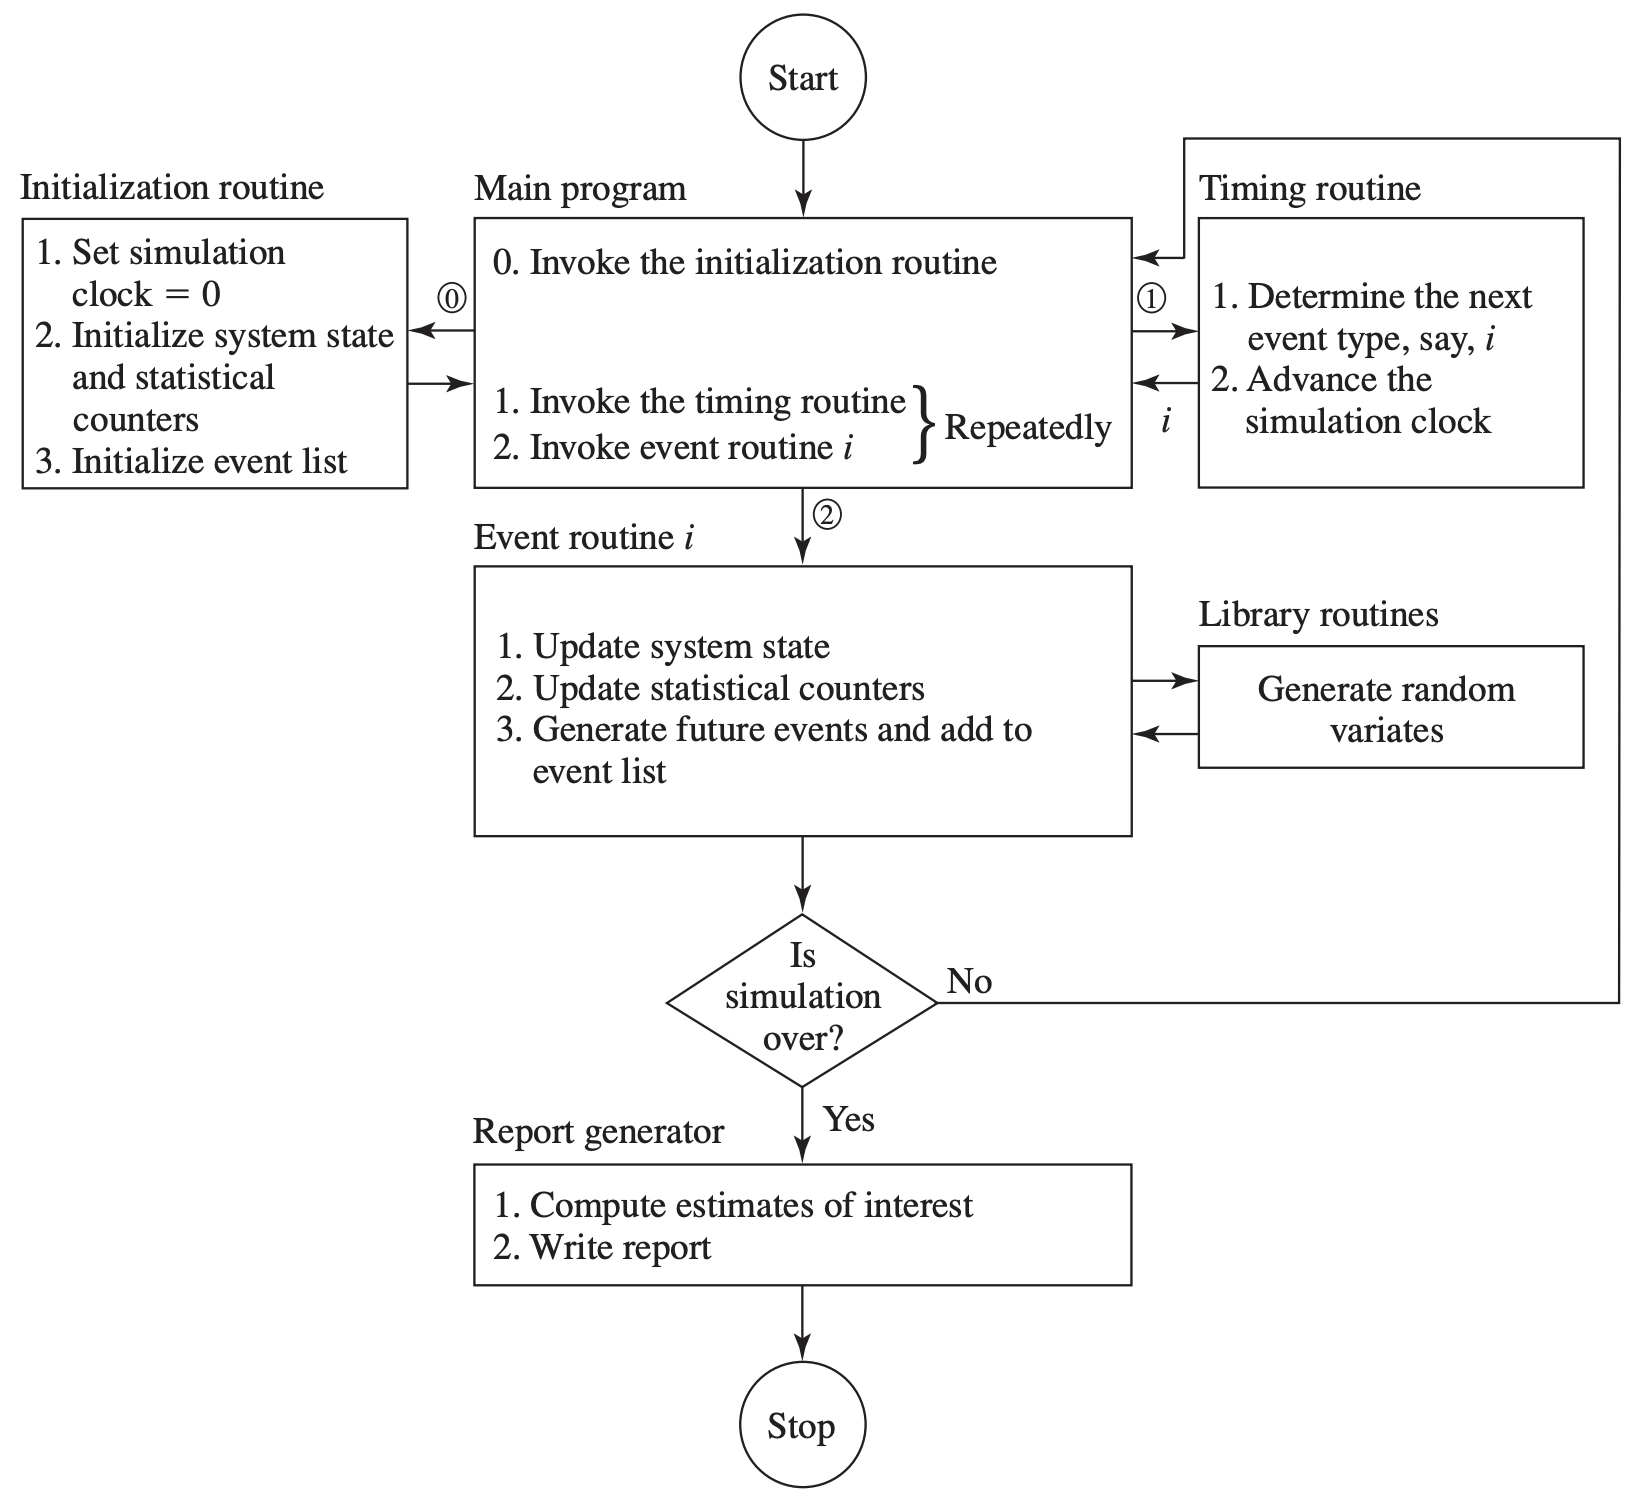
\includegraphics[width=.7\linewidth]{figures/discrete-event-simulation/time-advance-flow.png}
    \caption{Flusso di controllo dell'algoritmo Event-scheduling Time-advance \cite{Law15}.}
    \label{fig:next-event-flow}
\end{figure}

L'algoritmo in questione, il cui flusso di controllo è illustrato in figura~\ref{fig:next-event-flow} è suddiviso in tre sezioni chiave: \textit{inizializzazione}, \textit{ciclo di elaborazione degli eventi} e \textit{fase di output}.
La simulazione inizia al tempo 0, quando il \textit{main program} dà avvio alla simulazione invocando la \textit{initialization routine}, nella quale il clock viene settato a 0 e le entità e le variabili di stato sono inizializzate.
Il controllo torna poi al main program, il quale invoca una \textit{timing routine} per identificare il prossimo evento da eseguire.
La lista degli eventi futuri contiene tutti gli eventi ordinati per tempo di accadimento: $FEL = [t_1, t_2, \dots t_n], t_1 \leq t_2 \leq \dots \leq t_n$. 
Il tempo $t$ è il valore corrente del clock, mentre l'evento associato al tempo $t_1$ è chiamato evento imminente, ovvero il prossimo evento che dovrà verificarsi.~\cite{DBLP:books/daglib/0034857}
Il controllo torna nuovamente al main program, il quale invoca l'\textit{event routine} grazie al quale l'evento imminente viene eseguito effettivamente. 
L'esecuzione dell'evento imminente, al tempo $t$, seguita dalla generazione di uno snapshot correlato, comporta l'avanzamento del clock al successivo istante temporale, $t_1$. L'evento imminente è rimosso quindi dalla FEL ed eseguito, generando un nuovo snapshot a $t_1$ basato sulla natura dell'evento e lo snapshot precedente. In questa fase nuovi eventi futuri possono essere generati e aggiunti opportunamente alla FEL.
Il processo si ripete ciclicamente fino alla conclusione della simulazione. 
Durante la fase di output vengono invece elaborate e registrate le statistiche di interesse. 


\subsubsection{Gestione Future Event List}
Una Future Event List, come anticipato, è la struttura dati che contiene l'elenco degli eventi programmati per verificarsi in futuro. Tradizionalmente l'elenco è ordinato in base al tempo di esecuzione al quale l'evento è stato schedulato, ma questo non è un requisito. 
La gestione efficiente della FEL è di fondamentale importanza, alcuni modelli di simulazione impiegano più tempo CPU nella gestione della lista piuttosto che qualsiasi altro aspetto, come per esempio la generazione di numeri casuali, l'elaborazione di eventi, l'esecuzione di operazioni aritmetiche varie ecc\dots

Nella gestione degli eventi che compongono la FEL, ci sono due operazioni critiche: l'operazione di inserimento (\textit{enqueue}) e l'operazione di cancellazione (\textit{dequeue}). Un'operazione di cancellazione viene eseguita per elaborare l'evento o perché un evento, precedentemente pianificato deve essere annullato per qualche motivo. L'inserimento e la cancellazione possono verificarsi in una posizione prescritta nella lista degli eventi, oppure potrebbe essere necessario avviare una ricerca per determinare la giusta posizione. 
Importante è anche l'operazione di modifica, in cui una ricerca di evento esistente presente in lista è seguita da una modifica di qualche aspetto dell'evento stesso, come ad esempio la modifica del tempo di accadimento al quale è schedulato. 

Esistono tre criteri principali per determinare l'efficacia della struttura data e dell'algoritmo per la gestione della FEL: 
\begin{itemize}
    \item \textbf{Velocità}: la struttura dati e l'algoritmo per inserire ed eliminare un evento devono essere ottimizzate per minimizzare il tempo di esecuzione. Per ottenere tempi di esecuzione rapidi è fondamentale una ricerca degli eventi efficiente. Un algoritmo efficiente tende a limitare il numero di eventi ricercati per l'inserimento o la cancellazione. 
    \item  \textbf{Robustezza}: È necessaria una gestione efficace degli errori per affrontare scenari imprevisti. Occorre una validazione dei dati durante l'inserimento per garantire l'integrità della struttura dati.  
    \item \textbf{Adattabilità}: La FEL dovrebbe consentire la configurazione di parametri chiave per adattarsi a diverse modalità di gestione degli eventi o politiche temporali. Dovrebbe inoltre essere progettata in modo che nuove funzionalità o tipi di eventi possano essere facilmente integrati senza modificare drasticamente il codice esistente. 
\end{itemize}

\subsection{Partenza e terminazione}
Nella sezione precedente è stato descritto come la simulazione viene fatta partire e viene fatta terminare. Tipicamente per far partire una simulazione, in fase di inizializzazione viene generato un evento che viene poi inserito nella lista di eventi futuri. 
La terminazione può invece essere raggiunta tramite diversi meccanismi: 
\begin{itemize}
    \item Tempo di simulazione massimo: al tempo 0 viene schedulato un evento di stop ad un futuro tempo Te. In questo caso siamo certi che la simulazione verrà eseguita nell'intervallo $[0, T_e]$.
    \item Eventi speciali di terminazione: il tempo di esecuzione $T_e$ è determinato dalla simulazione stessa. In genere Te dipende dal numero di occorrenze di un determinato evento. Per esempio potrebbe essere il tempo del completamento del centesimo servizio presso un determinato centro di assistenza. 
    \item Terminazione quando la lista di eventi futuri è vuota.
\end{itemize}
Nel secondo e nel terzo caso il tempo per eseguire la simulazione non è conosciuto a priori e può variare di simulazione in simulazione.
Le esecuzioni di una simulazione possono essere classificate in transient e steady state La selezione del tipo di simulazione è particolarmente importante e la decisione deve essere presa in base all'output che vogliamo analizzare. Con il termine transient ci si riferisce ad una simulazione che termina, per causa di un evento speciale o ad un tempo prefissato. 
Una simulazione steady state, al contrario, non termina mai. L'obiettivo in questo caso è studiare il comportamento a lungo termine del sistema. 

\subsection{Distribuzioni di probabilità}
Il successo di una simulazione richiede un approccio completo che va oltre la semplice creazione di un diagramma di flusso del sistema in esame, la sua traduzione in un ``programma'' per computer e la replicazione di alcune configurazioni proposte del sistema. L'uso della probabilità e della statistica è un aspetto fondamentale di uno studio di simulazione, tanto che ogni team di modellazione dovrebbe includere almeno un esperto con una solida formazione in queste tecniche~\cite{Law15}.

Per effettuare una simulazione, utilizzando input casuali come i tempi di arrivo o le dimensioni della domanda, occorre specificare le loro distribuzioni di probabilità. La scelta delle corrette distribuzioni può determinare l'accuratezza del modello, spesso in modo drastico. 
Nelle simulazioni ad eventi discreti è comune modellare il tempo trascorso tra gli arrivi successivi degli eventi utilizzando distribuzioni di probabilità. 
Ad esempio, nel caso di una coda di attesa in un sistema di servizio, i tempi tra gli arrivi dei clienti possono essere modellati utilizzando una distribuzione esponenziale o di Poisson. Queste distribuzioni consentono di rappresentare realisticamente il processo di arrivo degli eventi e di stimare la frequenza con cui si verificano.
I tempi di servizio potrebbero essere costanti o probabilistici. Se i tempi sono completamente casuali, potrebbe essere necessario dover utilizzare una distribuzione esponenziale. Potrebbe anche accadere che i tempi di servizio siano costanti, ma una variabilità casuale causi fluttuazioni in modo negativo o positivo. Ad esempio, il tempo impiegato da un tornio per attraversare un albero di 10 centimetri dovrebbe essere costante. Tuttavia, il materiale potrebbe presentare lievi differenze di durezza o lo strumento potrebbe usurarsi. Qualsiasi evento potrebbe causare tempi di lavorazione diversi. In questi casi la distribuzione normale potrebbe descrivere il tempo di servizio~\cite{DBLP:books/daglib/0034857}.
Oltre ai tempi di arrivo e di servizio, le simulazioni possono coinvolgere altre variabili casuali che influenzeranno il comportamento del sistema: i ritardi tra l'arrivo di un evento e la sua elaborazione possono essere modellati utilizzando distribuzioni di probabilità per rappresentare il tempo impiegato per completare determinate attività o processi. 
\sidenote{da capire se spiegare anche tutte le distribuzioni di probabilità che potrebbero essere usate (divise in continue e discrete) in modo dettagliato. Da capire perchè forse diventa una spiegazione troppo da libro di testo. Da chiedere al prof.}

\subsection{Simulazione parallela}
La simulazione parallela a eventi discreti (PDES) si riferisce all'esecuzione di un singolo programma di simulazione a eventi discreti su un computer sfruttando il calcolo parallelo~\cite{DBLP:journals/cacm/Fujimoto90}. Distribuendo l'esecuzione di una simulazione su più processori, si cerca di ridurre notevolmente il tempo di esecuzione del modello, fino a un fattore pari al numero di processori. Questo concetto è valido in teoria, in realtà la legge di Amdahl stabilisce che il miglioramento della velocità di esecuzione di un programma parallelizzabile su un sistema multicore è limitato dalla frazione sequenziale del programma~\cite{DBLP:conf/afips/Amdahl67}. In altra parole, anche se una parte del programma può essere eseguita in modo parallelo, ci sarà sempre una parte sequenziale che non può essere parallelizzata. La legge di Amdahl può essere espressa con la seguente formula: 
$$
Speedup_{max} = \frac{1}{(1-P)+\frac{P}{N}}
$$
Dove: 
\begin{itemize}
    \item $Speedup_{max}$ è il miglioramento massimo della velocità di esecuzione ottenibile parallelizzando il programma. 
    \item $P$ è la frazione di codice che può essere parallelizzata. 
    \item $N$ è il numero di core disponibili.
\end{itemize}
Per esempio, se si sta simulando un modello militare di grandi dimensioni o una rete di comunicazione contenente migliaia di nodi, il tempo di esecuzione potrebbe essere eccessivo e si potrebbe prendere in considerazione la simulazione parallela. Un altro uso della simulazione parallela potrebbe essere il processo decisionale in tempo reale. Ad esempio, in un sistema di controllo del traffico aereo, potrebbe risultare utile simulare diverse ore di traffico aereo per decidere come reindirizzarlo al meglio~\cite{DBLP:conf/wsc/Wieland98}. 
Lo sviluppo di una simulazione parallela richiede la scomposizione del modello in processi logici (LP). I singoli LP sono assegnati a processori diversi, ognuno dei quali si occupa di simulare la propria parte di modello. Gli LP comunicano fra loro inviandosi messaggi o eventi con data e ora.
Quando si progetta una simulazione parallela è di fondamentale importanza garantire che gli eventi del modello, indipendentemente dal loro LP, vengano elaborati nella corretta sequenza temporale, mantenendo in questo modo l'ordine causale di essi. Se ogni LP elabora tutti i suoi eventi (generati da se stesso o da un altro LP) in ordine di tempo crescente, garantendo che gli eventi successivi siano eseguiti solo dopo quelli precedenti, e garantendo che gli eventi siano correttamente sincronizzati durante l'esecuzione in parallelo, allora l'ordine causale viene automaticamente conservato nella simulazione distribuita. Questo principio è cruciale per evitare inconsistenze e risultati non realistici.
Ogni LP può essere visto come un modello di simulazione sequenziale a eventi discreti, con le proprie variabili di stato locali, i propri eventi e il proprio clock.
Storicamente sono stati adottati due meccanismi di sincronizzazione differente: \textit{conservativo} e \textit{ottimistico}~\cite{DBLP:conf/wsc/Fujimoto95}.
Quando si utilizza un meccanismo conservativo l'obiettivo è evitare di violare il vincolo di causalità temporale. Ad esempio, si supponga che un particolare LP si trovi attualmente al tempo di simulazione 25 e sia pronto a elaborare il prossimo evento, che ha un tempo di 30. Il meccanismo di sincronizzazione deve assicurarsi che questo LP non riceva in seguito un evento da un altro LP con tempo di accadimento inferiore a 30. Pertanto, l'obiettivo è determinare quando è effettivamente sicuro elaborare un particolare evento. 
La sincronizzazione conservativa presenta due principali svantaggi: 
\begin{itemize}
    \item Non può sfruttare appieno il parallelismo disponibile: se l'evento A influenza in qualche modo l'evento B, allora A e B devono essere eseguiti in sequenza. Se il modello è tale per cui A influisce raramente B, allora A e B potrebbero essere elaborati in modo concorrente per la maggior parte del tempo.
    \item Non è robusta: una modifica apparentemente piccola del modello può inficiare le prestazioni. 
\end{itemize}
Nella sincronizzazione di tipo ottimistico, le violazioni del vincolo di causalità locale possono verificarsi, ma il meccanismo di sincronizzazione rileva le violazioni e le recupera. Anche in questo caso ogni LP simula la propria porzione di modello in avanti nel tempo, ma non aspetta di ricevere messaggi da altri processi. 
Il meccanismo di time-warp~\cite{DBLP:journals/toplas/Jefferson85} è il più noto approccio ottimistico. Se un LP riceve un messaggio che avrebbe dovuto essere ricevuto nel sup passato (e che quindi potrebbe influenzare le sue azioni da quel momento in poi), viene effettuato un rollback nell'LP ricevente che porta il suo clock all'ora del messaggio in arrivo.
Parte del lavoro annullato potrebbe consistere nell'invio di messaggi ad altri LP. L'invio di questi messaggi viene anch'esso annullato grazie all'invio del corrispondente anti-messaggio. L'invio di anti-messaggi può generare a sua volta rollback secondari negli LP di destinazione.
I meccanismi di sincronizzazione ottimistici possono sfruttare il parallelismo in modo migliore rispetto agli approcci conservativi, poiché non sono limitati dallo scenario peggiore. Tutta via presentano comunque alcuni svantaggi: 
\begin{itemize}
    \item Comportano costi computazionali maggiori legati all'esecuzione dei rollback. 
    \item Richiedono una maggiore quantità di memoria, poiché ogni lo stato di ogni LP deve essere salvato periodicamente per poter effettuare i rollback.
\end{itemize}


\subsection{Cenni Storici}
La storia delle simulazioni ad eventi discreti si estende per oltre mezzo secolo, risalendo ai primi anni dell'era informatica. La necessità di modellare e comprendere il comportamento dinamico dei sistemi complessi ha spinto i ricercatori a sviluppare metodologie e strumenti per simulare il funzionamento di tali sistemi.
Le radici concettuali delle simulazioni ad eventi discreti possono essere rintracciate nella teoria dei processi stocastici, che ha trovato applicazioni pratiche nell'ambito dell'ingegneria, della gestione delle operazioni aziendali e della logistica. Nel corso degli anni '50 e '60, con l'avvento dei primi computer e l'espansione dei linguaggi di programmazione, emersero i primi tentativi di simulare sistemi complessi utilizzando modelli basati su eventi discreti. Questi primi sforzi furono spesso limitati dalle risorse computazionali disponibili e dalle limitazioni dei linguaggi di programmazione dell'epoca.
Negli anni '60 e '70, con l'avanzamento della tecnologia informatica e l'introduzione di linguaggi di programmazione più potenti, come FORTRAN e ALGOL, la simulazione ad eventi discreti divenne sempre più praticabile e diffusa. Durante questo periodo furono sviluppati i primi linguaggi di programmazione specificamente progettati per la simulazione, come SIMSCRIPT~\cite{DBLP:journals/ibmsj/DimsdaleM64} e GPSS~\cite{DBLP:journals/tssc/HollandM68}, i quali permisero ai ricercatori di modellare e analizzare sistemi complessi in modo più efficace e efficiente.
Negli anni successivi, con il continuo avanzamento della tecnologia informatica e l'introduzione di nuovi concetti e metodologie, come la simulazione ad oggetti e la simulazione basata su agenti, le simulazioni ad eventi discreti hanno continuato a evolversi e a trovare sempre più applicazioni in una vasta gamma di settori. 
Molte aziende, in particolare nel settore manifatturiero, utilizzarono le simulazioni come strumento di supporto alle decisioni. 
A livello informatico il nuovo millennio è stato caratterizzato dalla potenza sempre crescente dei personal computer, dalla diminuzione del prezzo di questi ultimi e dal World Wide Web~\cite{DBLP:journals/jors/Robinson05}. Le simulazioni hanno cominciato a integrare intelligenza artificiale e machine learning per migliorare la previsione e l'ottimizzazione dei sistemi. Inoltre, la crescente disponibilità di dati in tempo reale ha portato all'adozione di approcci di simulazione ibrida che combinano modelli ad eventi discreti con dati reali per migliorare la precisione delle previsioni e delle decisioni.


\subsection{Aree di impiego}
\subsubsection{Sistemi di Produzione e Movimentazione dei Materiali}
I sistemi di produzione e movimentazione dei materiali rappresentano una delle applicazioni più importanti della simulazione. La simulazione è stata utilizzata con successo come supporto nella progettazione di nuove strutture produttive, magazzini e centri di distribuzione.
Le simulazioni ad eventi discreti sono utilizzate per condurre analisi sulla capacità di produzione degli impianti, considerando le specifiche delle risorse disponibili come macchinari, manodopera e materiali. Questo aiuta ad individuare sovraccarichi o sottoutilizzazioni delle risorse e a pianificare la capacità in modo efficiente. 
Oltre alla produzione, viene impiegata anche per ottimizzare la logistica, comprese le operazioni di movimentazione dei materiali, lo stoccaggio, il prelievo, il trasporto e la distribuzione. Questo comprende l'analisi della disposizione degli impianti, dei percorsi di movimentazione e delle politiche di gestione degli inventari per massimare l'efficienza complessiva e ridurre i costi operativi. 
I simulatori ad eventi discreti consentono di modellare anche i sistemi di trasporto e distribuzione dei materiali sia all'interno che all'esterno dell'impianto manifatturiero. Ciò include la pianificazione delle rotte di trasporto, l'ottimizzazione dei tempi di consegna e l'analisi dei flussi di traffico per garantire una distribuzione efficiente dei materiali.
Infine, è possibile valutare le performance attuali del sistema di produzione e movimentazione dei materiali e testare strategie di miglioramento. Questo può includere l'implementazione di nuove tecnologie, l'ottimizzazione dei processi o la riduzione degli sprechi, contribuendo a migliorare complessivamente l'efficienza e la produttività del sistema.


\subsubsection{Sistemi informatici}
La simulazione dei sistemi informatici consente di modellare e analizzare il comportamento di reti di computer, server e sistemi distribuiti. 
I simulatori possono essere utilizzati per valutare le prestazioni del sistema, misurare latenza di rete, analizzare il throughput e identificare eventuali bottleneck. Inoltre, consentono di simulare il carico di lavoro sui sistemi, aiutando a ridimensionare correttamente l'infrastruttura e a pianificare l'allocazione di risorse. 
È possibile simulare anche l'utilizzo di nuovi algoritmi o politiche di gestione delle risorse, come strategie di scheduling dei processi, politiche di gestione della memoria e politiche di gestione della rete.
Modellare scenari di fallimento e valutare l'impatto dei guasti, valutando l'impatto di questi ultimi sulle prestazioni del sistema e sulla disponibilità dei servizi, consente di valutare la tolleranza ai guasti di sistemi informatici complessi. 
Anche la sicurezza del sistema può essere valutata, simulando scenari di minaccia e attacchi informatici, così da identificare eventuali vulnerabilità.

\subsubsection{Reti Informatiche}
La simulazione di reti informatiche consente di comprendere il comportamento dinamico delle reti, consentono di valutare le prestazioni della rete, misurando parametri chiave come la latenza e il throughput. Questo permette di identificare e risolvere eventuali punti critici che potrebbero compromettere le prestazioni della rete. 
Studiando il traffico di rete è possibile individuare possibili congestioni di rete e adottare strategie di routing per garantire una gestione efficiente delle risorse. 
Un altro aspetto importante è la possibilità di valutare la scalabilità della rete, ovvero la sua capacità di gestire un aumento del carico di lavoro o del numero di utenti. 
Il testing di nuovi protocolli e tecnologie consente di valutare le prestazioni di nuove soluzioni prima della loro effettiva implementazione su larga scala. 
Anche in questo caso, modellando scenari di attacco e valutando la robustezza delle contromisure di sicurezza adottate, è possibile analizzare la sicurezza della rete, proteggendola da minacce esterne e garantendo la sicurezza dei dati sensibili. 
%----------------------------------------------------------------------------------------
% BIBLIOGRAPHY
%----------------------------------------------------------------------------------------

\backmatter

%\nocite{*} % comment this to only show the referenced entries from the .bib file

\bibliographystyle{alpha}
\bibliography{bibliography}

\end{document}